\documentclass{report}
\usepackage{ctex}
\usepackage{graphicx}
\usepackage{amsmath}
\title{分光计的调节与使用A}
\author{王启骅 PB20020580}
\begin{document}
	\maketitle
	\section{实验目的}
1.学习分光计的调节与使用。\\
2.用分光计测量三棱镜的顶角大小与绿谱线的最小偏向角,从而算出三棱镜的折射率。
	\section{实验原理}
1.先调节分光计,(1)目测粗调望远镜水平,载物台水平。\quad(2)目镜调焦
这是为了使眼睛通过目镜看到分划板上的刻线。\quad(3) 调望远镜对平行光聚焦。\\
\quad(4) 调整望远镜光轴垂直仪器主轴\\
2.用最小偏向法测量三棱镜材料的折射率。\\
测量三棱镜顶角大小:
首先分别令三棱镜顶角A两平面正对望远镜,测得A的补角\\
$ \phi=\frac{1}{2}[|\theta_1-\theta_1'|+|\theta_2-\theta_2'|] $ \\
$   A=\pi-\phi $\\
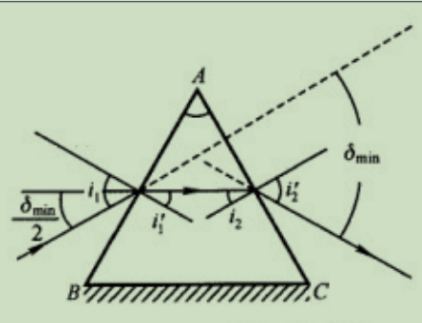
\includegraphics{1}\\
一束单色光以$ i_1 $角入射到AB面上,经棱镜两次折射后,从AC面折射出来,出射角为$ i_2' $。入射光和出射光之间的夹角$ \delta $称为偏向角。当棱镜顶角A一定时,偏向角$ \delta $的大小随入射角i1的变化而变化。当$ i_1=i_2' $时,$ \delta $为最小。这时的偏向角称为最小偏向角,记作$ \delta_{min} $。
\begin{center}
	$ i_1'=A/2 $\\
	$ \delta_{min}/2=i_1-i_1'=i_1-A/2 $\\
	$ i_1=\dfrac{A+\delta_{min}}{2} $\\
\end{center}
	则折射率为$ n=\dfrac{sin(\dfrac{A+\delta_{min}}{2})}{sin(A/2)} $
	\section{实验仪器}
	分光计,汞灯,双面镜,三棱镜
	\section{实验数据}
	\begin{flushleft}
		
	
	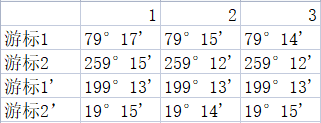
\includegraphics{2}	\\表1:三棱镜顶角测量原始数据\\
	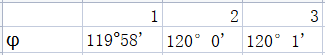
\includegraphics{4}\\表2:A补角的计算数据 \\
	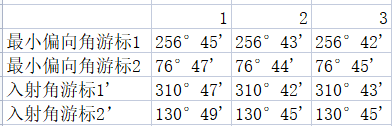
\includegraphics{3}\\表3:绿谱线最小偏向角测量原始数据\\
	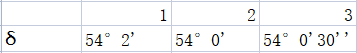
\includegraphics{5}\\表4:绿谱线最小偏向角计算数据\\
\end{flushleft}
	
	\section{数据处理与误差分析}
	顶角测量:$\bar{\phi}=\frac{1}{2}[|79^{\circ}17'-199^{\circ}13'|+|259^{\circ}15'-19^{\circ}15'|+|79^{\circ}15'-199^{\circ}13'|+|259^{\circ}12'-19^{\circ}14'|+|79^{\circ}14'-199^{\circ}13'|+|259^{\circ}12'-19^{\circ}15'|]/3=119.994^{\circ}$\\
	$\sigma_{\phi}=\sqrt{\dfrac{\sum_{i=1}^{3}(\phi_i-\bar{\phi})^2}{3-1}}$ \\ $ =\sqrt{\dfrac{(119^{\circ}58'0''-119^{\circ}59'40'')^2+(120^{\circ}0'0''-119^{\circ}59'59'')^2+(120^{\circ}1'0''-119^{\circ}59'40'')^2}{2}}=0.025^{\circ}$
	\\
	$ \Delta_B=1' $\\
	$ U_{\phi}=U_{A}=\sqrt{(t_{0.95}\frac{\sigma_{\phi}}{\sqrt{n}})^2+(k_p\frac{\Delta_B}{C})^2}=\sqrt{(4.30\times0.025^{\circ}/\sqrt{3})^2+(1.645\times1'/\sqrt{3})^2}=0.06^{\circ},P=0.95 $\\
	$ A=(60.01\pm0.06)^{\circ} $\\
	最小偏向角测量:
	$ \bar{\delta}=\dfrac{54^{\circ}2'+54^{\circ}0'+54^{\circ}0'30''}{3}=54^{\circ}0'50'' $\\
	$ \sigma_{\delta}=\sqrt{\dfrac{\sum_{1}^{3}(\delta_i-\bar{\delta})^2}{3-1}}=0.017^{\circ} $\\
		$ \Delta_B=1' $\\
	$
	 U_{\delta}=\sqrt{(t_{0.95}\frac{\sigma_{\delta}}{\sqrt{n}})^2+(k_p\frac{\Delta_B}{C})^2}=\sqrt{(4.30\times0.017^{\circ}/\sqrt{3})^2+(1.645\times1'/\sqrt{3})^2}=0.05^{\circ},P=0.95 $\\
	$ \delta=(54.01\pm0.05)^{\circ} $\\
	$ U_n/n=\sqrt{(\dfrac{|cos(\frac{A+\delta}{2})|\sqrt{1/4((U_A/A)^2+(U_{\delta}/\delta)^2)}}{sin(\frac{A+\delta}{2})})^2+(\dfrac{|cos(A/2)|\frac{U_A/A}{2}}{sin(A/2)})^2}=1\times10^{-3} $\\
	折射率$ n=1.6773\pm0.0017 $
	
	
	
	
	\section{实验讨论}
在实验过程中,要注意游标盘两游标的顺序,不要把游标读数顺序搞反了,导致计算结果错误。在进行测量三棱镜顶角时,三棱镜反射率较低,要在尽量暗的环境中测量,否则很难看到十字叉丝。
	\section{思考题}
不是。由于进行望远镜垂直于主轴调节时,只进行了载物台的两个螺钉的调节。当经过载物台两个螺钉的调节后,可以使双面镜此时的位置保证双面镜平面平行于主轴,但是载物台平面可能并不水平,导致在不同位置再次放上双面镜时,双面镜镜面不与主轴相平行,而此时望远镜仍是与主轴垂直的。此时应该调节载物台的第三个螺钉使载物台水平,而不应调节望远镜。
	
\end{document}